\documentclass{report}

\usepackage{graphicx}
\usepackage{cancel}
\usepackage{amsmath}
\usepackage{ragged2e}
\usepackage{arcs}
\usepackage{nopageno}
\usepackage[utf8]{inputenc}
\usepackage[english,russian]{babel}
\usepackage[a4paper, left=0.4cm, top=0.5cm, right=0.4cm, bottom=0.5cm]{geometry}




\begin{document}


\noindent
\textbf{Векторная функция} векторного аргумента -- это соответствие $r$, при котором
$\forall$ точке $x \in \Omega$ евклидова пространства $R^{m}$ сопостовляется 
вектор $r(x)$ множества $Q$ евклидова пространства $R^{p}$.\\
$x \in \Omega = \{(x_1, \ldots, x_m)\} \subset R^{m} \to r(x)
\in Q = \{(r_1, \ldots, r_p)\} \subset R^{p}$\\
При этом множество $\Omega$ область задания, а $Q$ множество значений.
Если $\Omega = \{x\}$ -- множество точек на прямой, то имеем функцию одного
скалярного аргумента $r(x)$.\\
Если $\Omega = \{(x_1, \ldots, x_m)\} \subset R^{m}$ -- множество точек евклидова
пространства, то имеем векторную функцию нескольких скалярных
аргументов $r(x_1, \ldots, x_m)$.\\

\noindent
\textbf{Годограф векторной функции}\\
Пусть $(r_1, \ldots, r_p)$ -- координаты $r(x) \in Q \subset R^{p}$.
Задание векторной функции $r(x)$ равносильно заданию скалярных функций\\
$r_1(x_1, \ldots, x_m), \ldots, r_p(x_1, \ldots, x_m)$, и если начала этих
векторов совместить с началом соответствующей ДПСК, то точечное множество концов
рассматриваемых радиус векторов будем называть годографом векторной функции.\\
If p = 3 годограф векторной функции есть кривая, p = 2 -- поверхность.\\


\noindent
\textbf{Способы задания кривых}\\
\indent Элементарной кривой называют множество точек пространства, являющееся
образом отрезка при топологическом отображении его в пространство.\\
Точки соответствующие конечным точкам отрезка, называют конечными точками
элементарной кривой. Элементарные кривые -- примыкающие если одна или обе
пары их конечных точек совпадают между собой.\\
Кривой линией называется множество точек пространства, которое состоит
из конечного или счетного множества элементарных кривых, примыкающих друг к другу.\\
\indent Пусть $\gamma$ -- элементарная кривая, являющаяся образом промежутка 
$a < t < b$ при топологическом отображении f его в пространство $R^{3}$.
$x(t),\ y(t),\ z(t)$ -- координаты точки на кривой $\gamma$ соответствующей
значению $t \in (a, b)$.\\
Тогда систему равенств $x(t),\ y(t),\ z(t),\ t \in (a, b)$ называют уравнениями кривой 
$\gamma$ в параметрической форме или параметризацией кривой (кривая $\gamma$ параметризована
этими уравнениями).\\
Если же считать $x(t),\ y(t),\ z(t)$ координатами радиус-вектора $\overrightarrow{r}(t)$
соответствующей точки кривой $\gamma$, мы получим векторную функцию $\overrightarrow{r}(t),\ $
$t \in (a, b)$, годографом которой является данная кривая. (способ задания кривой через векторную
функцию скалярного аргумента по сути эквивалентный параметрическому способу).\\
Допустим, что кривая $\gamma$ задается векторной функцией $\overrightarrow{r}(t),\ t \in (a, b)$.\\
Тогда заменив параметр $t$ параметром $u$ через отношение $t = g(u),\ u \in (\alpha, \beta),$ где $g$
-- строго возрастающая и непрерывная функция. Тогда получится новая параметризация, одну кривую
можно задать множеством параметризаций.\\

\noindent
\textbf{Касательная к кривой}\\
Пусть $\gamma$ -- некторая кривая, $P$ -- фиксированная точка и $M$ -- подвижная точка на кривой
$\gamma,\ PM$ -- хорда кривой.\\
Прямая $PM$ стремится к прямой $PT$ при $M \to P$, если угол $\phi$ между этими прямыми стремится
к нулю, когда $M \to P$.\\
Касательной к кривой $\gamma$ в точке $P$ называют прямую $PT$, к которой стремится хорда $PM$,
когда $M \to P$.\\
\begin{figure}[ht!]
\centering
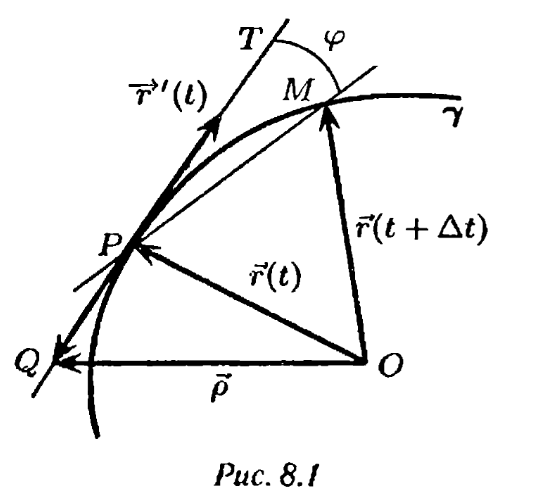
\includegraphics[width=60mm]{curve.png}
\end{figure}

\noindent
\textbf{Нормальной плоскостью кривой} в точке $P$ называется плоскость, проходящая через точку
$P$ перпендикулярно касательной в данной точке.\\
Векторное уравнение нормальной плоскости $\pi$ в точке $P(\overrightarrow{r}(t))$ имеет вид:
$(\overrightarrow{\rho} - \overrightarrow{r}(t)) \cdot \overrightarrow{r}'(t) = 0$, где 
$\overrightarrow{\rho}$ -- радиус-вектор произвольной точки плоскости $\pi$.\\

\newpage
\noindent
\textbf{Соприкасающаяся плоскость}\\
Пусть $\gamma$ -- некоторая кривая, $P \in \gamma$ -- фиксированная точка, $M \in \gamma$ --
подвижная, $PT$ -- касательная к кривой в точке $P$, $PTM$ -- плоскость проведенная через
касательную $PT$ и точку $M$.\\
Плоскость $RTM$ стремится к плоскости $\pi$ при $M \to P$, если угол между этими плоскостями
стремится к нулю, когда $M \to P$.\\
Плоскость $\pi$, к которой стремится плоскость $PTM$, когда $M \to P$, называют
соприкасающейся плоскостью кривой $\gamma$ в точке $P$.\\
\begin{figure}[ht!]
\centering
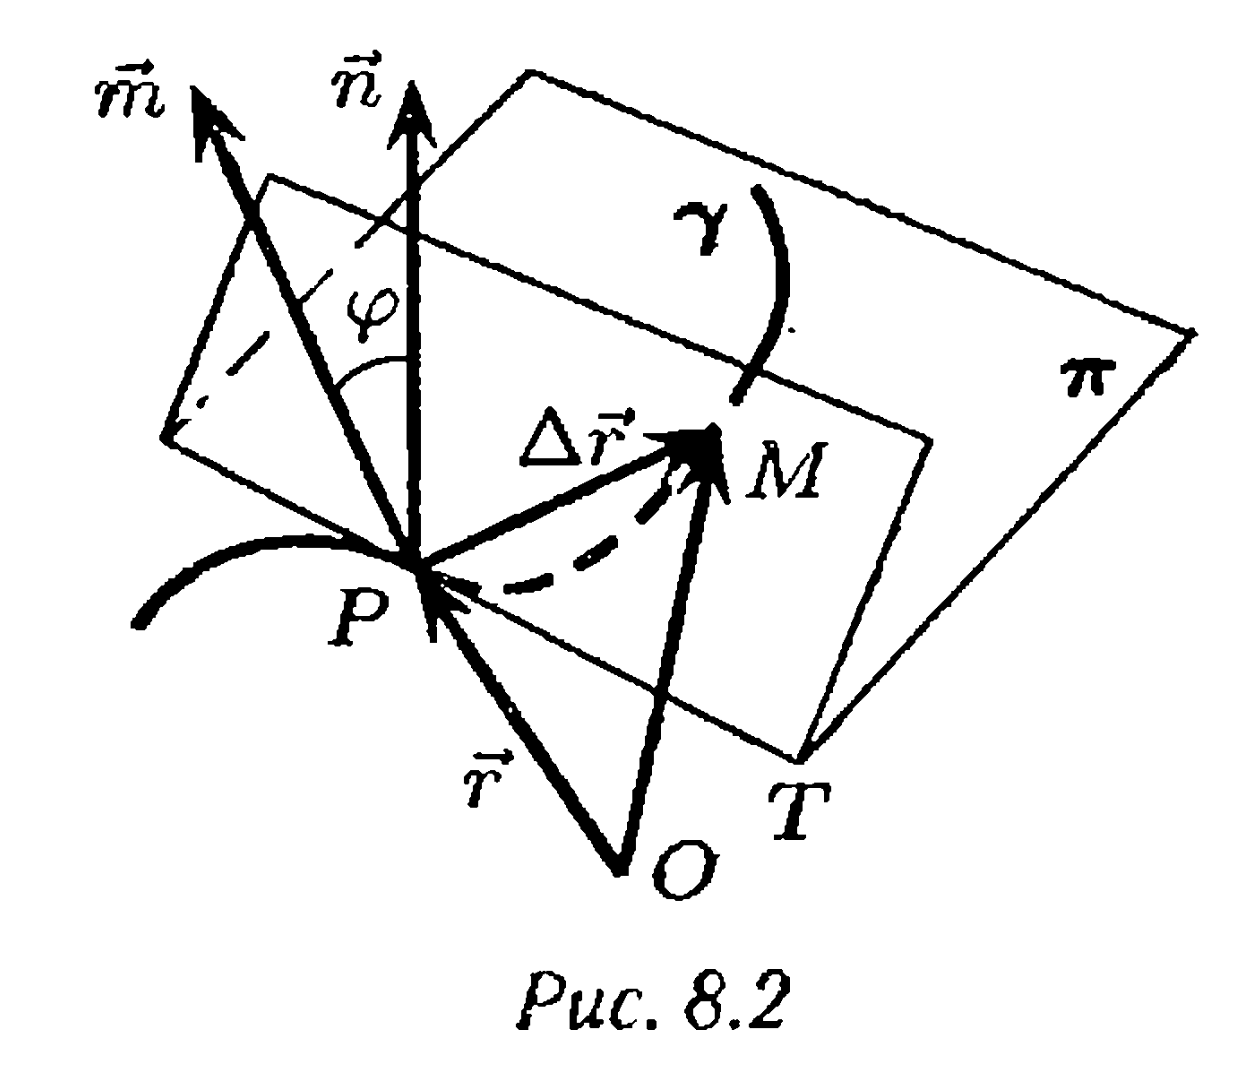
\includegraphics[width=60mm]{curve2.png}
\end{figure}


\noindent
\textbf{Спрямляющая плоскость, главная нормаль, бинормаль}\\
Прямую проходящую через точку $P$ перпендикулярно касательной кривой,
называют нормалью кривой. $(CD, MN)$\\ 
Нормаль, лежащую в соприкасающейся плоскости кривой,
называют главной нормалью кривой. $(CD)$\\
Нормаль, перпендикулярную соприкасающейся плоскости кривой,
называют бинормалью кривой. $(MN)$\\
Плоскость, определяемую касательной к кривой и бинормалью, 
называют спрямляющей плоскостью. $(\pi_3)$\\
\begin{figure}[ht!]
\centering
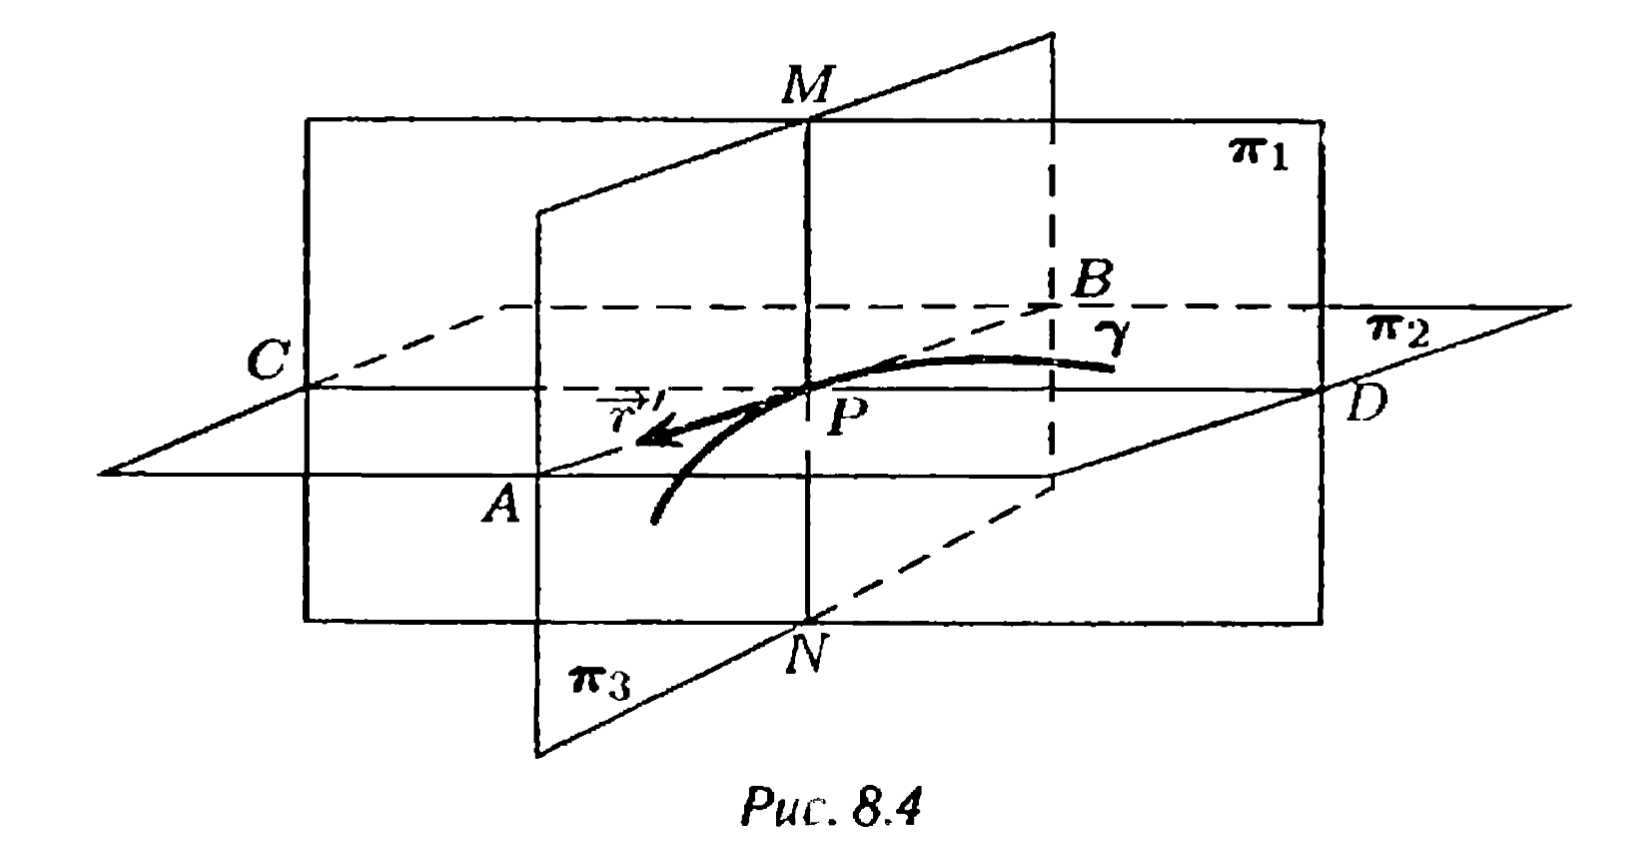
\includegraphics[width=90mm]{curve3.png}
\end{figure}


\noindent
\textbf{Длина дуги кривой}\\
Пусть $\gamma = \overarc{AB}$ -- дуга кривой, являющаяся образом замкнутого отрезка
$[a, b]$ при топологическом отображении.\\
Разобьем дугу $AB$ на $n$ частичных дуг точками:\\


\end{document}
